\documentclass[11pt]{beamer}

% Theme & Typography
\usetheme{Madrid}
\usecolortheme{beaver}
\usefonttheme{professionalfonts}

% Custom Colors (Beaver Palette Alignment)
\definecolor{darkred}{RGB}{160, 20, 20}
\definecolor{darkblue}{RGB}{20, 40, 140}
\definecolor{darkgreen}{RGB}{20, 120, 40}

% Packages
\usepackage[T1]{fontenc}
\usepackage[utf8]{inputenc}
\usepackage{lmodern}
\usepackage[scaled=0.88]{inconsolata}
\usepackage{amsmath,amssymb,amsthm}
\usepackage{graphicx}
\usepackage{hyperref}
\usepackage{tikz}
\usetikzlibrary{arrows,arrows.meta,positioning,shapes,calc,fit,backgrounds}
\usepackage{listings}
\usepackage{booktabs}
\usepackage{array}

% Semantic Domain Macros
\providecommand{\OWN}{\textbf{OWN}}
\providecommand{\UP}{\textbf{UP}}
\providecommand{\HEAP}{\textbf{HEAP}}
\providecommand{\retParams}{\text{retParams}}
\providecommand{\ROOT}{\text{ROOT}}
\providecommand{\GLOBAL}{\text{GLOBAL}}
\providecommand{\dom}{\mathrel{\text{dom}}}
\providecommand{\idom}{\text{idom}}

% Code Listing Configuration (Modern Fluent Style)
\lstdefinestyle{javacode}{
  language=Java,
  basicstyle=\fontsize{7.5pt}{9.5pt}\selectfont\ttfamily,
  keywordstyle=\color{blue!80!black}\bfseries,
  commentstyle=\color{black!50}\slshape,
  stringstyle=\color{darkgreen},
  showstringspaces=false,
  breaklines=true,
  columns=flexible,
  keepspaces=true,
  frame=single,
  frameround=tttt,
  rulecolor=\color{blue!30!black!20},
  backgroundcolor=\color{blue!2!gray!6},
  xleftmargin=3pt,
  xrightmargin=3pt,
  framesep=3pt,
  numbers=none,
  tabsize=2
}

\lstdefinestyle{javacodetiny}{
  language=Java,
  basicstyle=\fontsize{6.6pt}{8.4pt}\selectfont\ttfamily,
  keywordstyle=\color{blue!80!black}\bfseries,
  commentstyle=\color{black!50}\slshape,
  stringstyle=\color{darkgreen},
  showstringspaces=false,
  breaklines=true,
  columns=flexible,
  keepspaces=true,
  frame=single,
  frameround=tttt,
  rulecolor=\color{blue!30!black!20},
  backgroundcolor=\color{blue!2!gray!6},
  xleftmargin=3pt,
  xrightmargin=3pt,
  framesep=3pt,
  numbers=none,
  tabsize=2
}

\lstdefinestyle{jimplecode}{
  basicstyle=\fontsize{6.6pt}{8.4pt}\selectfont\ttfamily,
  keywordstyle=\color{purple!90!black}\bfseries,
  commentstyle=\color{black!50}\slshape,
  stringstyle=\color{orange!80!black},
  showstringspaces=false,
  breaklines=true,
  columns=flexible,
  keepspaces=true,
  frame=single,
  frameround=tttt,
  rulecolor=\color{purple!30!black!20},
  backgroundcolor=\color{purple!2!gray!6},
  xleftmargin=3pt,
  xrightmargin=3pt,
  framesep=3pt,
  numbers=none,
  tabsize=2
}

% Beamer Block Tweaks
\setbeamertemplate{navigation symbols}{}
\setbeamertemplate{blocks}[rounded][shadow=true]

% Footline: Chapter Name out of 5 Chapters at Bottom Right
\setbeamertemplate{footline}{%
  \leavevmode%
  \hbox{%
  \begin{beamercolorbox}[wd=.33\paperwidth,ht=2.25ex,dp=1ex,center]{author in head/foot}%
    \usebeamerfont{author in head/foot}\insertshortauthor
  \end{beamercolorbox}%
  \begin{beamercolorbox}[wd=.33\paperwidth,ht=2.25ex,dp=1ex,center]{title in head/foot}%
    \usebeamerfont{title in head/foot}\insertshorttitle
  \end{beamercolorbox}%
  \begin{beamercolorbox}[wd=.33\paperwidth,ht=2.25ex,dp=1ex,leftskip=1ex,rightskip=1ex]{date in head/foot}%
    \hfill%
    \usebeamerfont{date in head/foot}%
    \ifnum\thesection>0%
      \insertsectionhead%
    \fi%
    \hfill%
    \insertframenumber/\inserttotalframenumber%
  \end{beamercolorbox}}%
  \vskip0pt%
}

% Header Logo Integration
\addtobeamertemplate{frametitle}{}{%
  \begin{tikzpicture}[remember picture,overlay]
    \node[anchor=north east, xshift=-0.2cm, yshift=-0.1cm] at (current page.north east) {%
      
\includegraphics[height=0.62cm]{iitb_logo.png}%
    };
  \end{tikzpicture}%
}

% Title & Author Metadata
\title[DOSA: Static Ownership Inference]{Binding Object Lifetimes for Improved Garbage Collection in Java}
\subtitle{CS492 BTP 1 Presentation}

\author[Harshil Solanki]{%
  \textbf{Presented by:}\\[0.15em]
  \textcolor{darkred}{\textbf{Harshil Solanki}}\\[0.45em]
  \textbf{Supervised by:}\\[0.15em]
  \textbf{Prof. Manas Thakur}\\[0.3em]
  \small Department of Computer Science \& Engineering\\
  \small Indian Institute of Technology Bombay
}

\institute[IIT Bombay]{IIT Bombay}
\date{24 November 2026}
\titlegraphic{
\includegraphics[height=0.9cm]{iitb_logo.png}}

\begin{document}

% ==============================================================================
% TITLE & OUTLINE
% ==============================================================================
\begin{frame}[plain]
  \titlepage
\end{frame}

\begin{frame}{Presentation Structure}
  \setbeamertemplate{section in toc}[sections numbered]
  \tableofcontents
\end{frame}

% ==============================================================================
% SECTION 1: MOTIVATION & EXPLORATORY TRAJECTORY
% ==============================================================================
\section[Motivation \& Background]{Motivation \& Exploratory Trajectory}

\begin{frame}{The Memory Management Dilemma in Managed Languages}
  \begin{itemize}
    \item \textbf{Garbage Collection (GC) Trade-Off:}
      \begin{itemize}
        \item Automatic memory management provides memory safety, but introduces tracing pauses and throughput overhead.
        \item High-throughput and interactive workloads experience latency variability driven by stop-the-world GC sweeps.
      \end{itemize}
    \item \textbf{Lifetimes in Systems Languages:}
      \begin{itemize}
        \item Modern languages (e.g., Rust) demonstrate compile-time lifetime and ownership tracking without tracing GC.
        \item \textbf{Central Question:} Can ahead-of-time static analysis infer method-scoped lifetimes in unmodified Java bytecode?
      \end{itemize}
  \end{itemize}
  
  \begin{block}{Thesis Statement}
    \small
    Ahead-of-time ownership inference can identify method-scoped object clusters in Java bytecode, enabling bulk object reclamation at method return without programmer annotations. \textit{Automated, Method-associated memory management}.
  \end{block}
\end{frame}

\begin{frame}{Prior Art \& Practical Limitations in Java}
  \begin{columns}[T]
    % Left Column: Visual Call-and-Return Dilemma
    \begin{column}{0.37\textwidth}
      \begin{block}{Cross-Frame Return Dilemma}
        \centering
        \vspace{0.1em}
        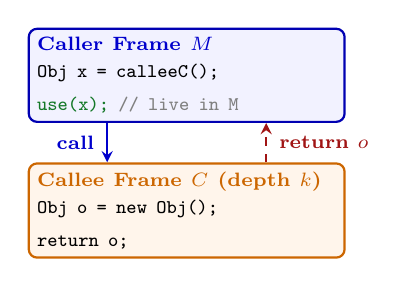
\begin{tikzpicture}[
          framebox/.style={rectangle, draw=blue!70!black, fill=blue!5, rounded corners=3pt, thick, text width=3.8cm, inner sep=3pt},
          calleebox/.style={rectangle, draw=orange!80!black, fill=orange!8, rounded corners=3pt, thick, text width=3.8cm, inner sep=3pt},
          edge/.style={->, >=stealth, thick}
        ]
          % Caller frame M
          \node[framebox] (caller) {
            {\scriptsize\bfseries\color{blue!80!black} Caller Frame $M$}\\[1pt]
            {\fontsize{7.2pt}{8.8pt}\selectfont\ttfamily
            Obj x = calleeC();\\
            \color{darkgreen}use(x); \color{black!50}// live in M}
          };

          % Callee frame C
          \node[calleebox, below=0.5cm of caller] (callee) {
            {\scriptsize\bfseries\color{orange!80!black} Callee Frame $C$ (depth $k$)}\\[1pt]
            {\fontsize{7.2pt}{8.8pt}\selectfont\ttfamily
            Obj o = \textbf{new} Obj();\\
            \textbf{return} o;}
          };

          % Arrows between M and C
          \draw[edge, blue!80!black] ($(caller.south west)!0.25!(caller.south east)$) -- 
            node[midway, left=1pt, font=\scriptsize\bfseries] {call}
            ($(callee.north west)!0.25!(callee.north east)$);
          \draw[edge, darkred, dashed] ($(callee.north west)!0.75!(callee.north east)$) -- 
            node[midway, right=1pt, font=\scriptsize\bfseries] {return $o$}
            ($(caller.south west)!0.75!(caller.south east)$);
        \end{tikzpicture}

        \vspace{0.2em}
        \raggedright
        \scriptsize
        \begin{itemize}\setlength{\itemsep}{1.5pt}\setlength{\parsep}{0pt}
          \item Object $o$ outlives $C$, but is dead when caller $M$ returns.
          \item \textbf{Lexical free at $C$:} Dangling pointer in $M$.
          \item \textbf{HotSpot Intra-EA:} Callee return forces heap fallback.
        \end{itemize}
      \end{block}
    \end{column}

    % Right Column: Structured Comparison Matrix
    \begin{column}{0.59\textwidth}
      \scriptsize
      \setlength{\tabcolsep}{2.5pt}
      \renewcommand{\arraystretch}{1.14}
      \begin{tabular}{@{}l >{\raggedright\arraybackslash}p{1.55cm} >{\raggedright\arraybackslash}p{3.05cm}@{}}
        \toprule
        \textbf{Paradigm} & \textbf{How Scope Is Defined} & \textbf{Limitation in Java} \\
        \midrule
        \shortstack[l]{\textbf{Ownership}\\{\fontsize{4.8pt}{5.6pt}\selectfont\textit{(AliasJava, Universe Types)}}} & Static types (\texttt{@Rep}) & Pervasive manual annotations; unannotated bytecode unsupported \\
        \addlinespace[1.5pt]
        \textbf{Lexical} & Block LIFO (\texttt{letregion}) & Cross-scope return causes dangling pointer or memory leak \\
        \addlinespace[1.5pt]
        \textbf{Intra-EA} & Method graph (C2) & Binary escape: callee return forces global heap allocation \\
        \addlinespace[1.5pt]
        \textbf{Gupta '26} & Backward DFS ($k \le 2$) & Search cutoff at $k>2$; static field escapes unhandled \\
        \midrule
        \textbf{DOSA} & \textbf{Dominator Tree} & \textcolor{darkgreen}{\textbf{Solved:}} Bounded by $M$ region; zero manual syntax \\
        \bottomrule
      \end{tabular}
    \end{column}
  \end{columns}
\end{frame}

\begin{frame}{Diagnostic Escape Auditing: Uncovering Root Causes}
  \footnotesize We built an out-of-lattice \textbf{diagnostic auditing engine} to trace why objects escape:

  \begin{columns}[T]
    \begin{column}{0.48\textwidth}
      \begin{block}{Stava Attribution Barriers}
        \scriptsize
        \begin{itemize}\setlength{\itemsep}{1pt}
          \item \textbf{Absorbing Lattice:} Status collapses to singleton \texttt{Escape}, erasing conditional values.
          \item \textbf{Severed Attribution:} Returns map to synthetic placeholder $\langle\text{returnValue}, 0\rangle$.
        \end{itemize}
      \end{block}
    \end{column}

    \begin{column}{0.48\textwidth}
      \begin{block}{Decoupled Diagnostic Engine}
        \scriptsize
        \begin{itemize}\setlength{\itemsep}{1pt}
          \item \textbf{Decoupled Side Map $\mathcal{R}$:} Append-only log preserving fixed-point convergence.
          \item \textbf{Concrete Stamping:} Traces returns to real allocation bytecode indices ($bci$).
        \end{itemize}
      \end{block}
    \end{column}
  \end{columns}

  \begin{exampleblock}{Diagnostic Attribution: Recovering Hidden Causes}
    \scriptsize
    \textbf{Bytecode Stmt:} \texttt{Config.buffer = new StringBuffer();} (at bytecode index 28)\\
    \textbf{Upstream Stava:} Discards attribution $\implies$ status collapses to singleton \texttt{Escape}\\
    \textbf{Our Side Map $\mathcal{R}$:} Retains trigger $\implies$ $\mathcal{R}[\texttt{Config}][\text{bci } 28] = \{\texttt{STATIC\_FIELD\_STORE } (\texttt{Config.buffer})\}$
  \end{exampleblock}
\end{frame}
\begingroup
\setbeamerfont{block title}{size=\scriptsize}
\begin{frame}{Observation: Escape Distribution \& Motivations}
  \centering
  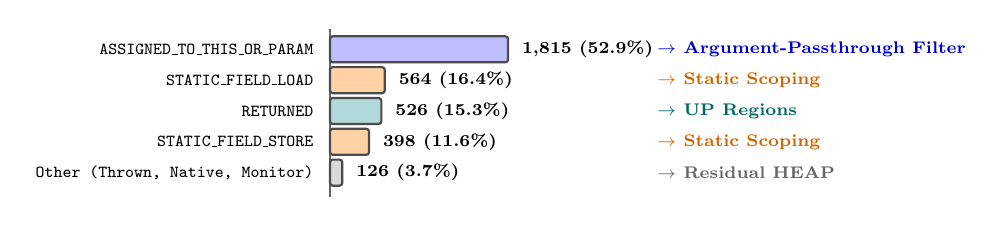
\begin{tikzpicture}[
      scale=0.87, every node/.style={transform shape},
      bar/.style={draw=black!70, thick, rounded corners=1pt},
      lbl/.style={font=\scriptsize\ttfamily\bfseries, anchor=east},
      val/.style={font=\scriptsize\bfseries, anchor=west},
      target/.style={font=\scriptsize\bfseries, anchor=west}
  ]
    % Baseline
    \draw[thick, black!60] (0, -0.30) -- (0, 2.15);

    % Y=1.85: ASSIGNED_TO_THIS_OR_PARAM
    \node[lbl] at (-0.12, 1.85) {ASSIGNED\_TO\_THIS\_OR\_PARAM};
    \filldraw[bar, fill=blue!25] (0, 1.66) rectangle (2.60, 2.04);
    \node[val] at (2.68, 1.85) {1,815 (52.9\%)};
    \node[target, text=blue!80!black] at (4.65, 1.85) {$\rightarrow$ Argument-Passthrough Filter};

    % Y=1.40: STATIC_FIELD_LOAD
    \node[lbl] at (-0.12, 1.40) {STATIC\_FIELD\_LOAD};
    \filldraw[bar, fill=orange!35] (0, 1.21) rectangle (0.80, 1.59);
    \node[val] at (0.88, 1.40) {564 (16.4\%)};
    \node[target, text=orange!80!black] at (4.65, 1.40) {$\rightarrow$ Static Scoping};

    % Y=0.95: RETURNED
    \node[lbl] at (-0.12, 0.95) {RETURNED};
    \filldraw[bar, fill=teal!30] (0, 0.76) rectangle (0.75, 1.14);
    \node[val] at (0.83, 0.95) {526 (15.3\%)};
    \node[target, text=teal!80!black] at (4.65, 0.95) {$\rightarrow$ \UP{} Regions};

    % Y=0.50: STATIC_FIELD_STORE
    \node[lbl] at (-0.12, 0.50) {STATIC\_FIELD\_STORE};
    \filldraw[bar, fill=orange!35] (0, 0.31) rectangle (0.57, 0.69);
    \node[val] at (0.65, 0.50) {398 (11.6\%)};
    \node[target, text=orange!80!black] at (4.65, 0.50) {$\rightarrow$ Static Scoping};

    % Y=0.05: Other
    \node[lbl] at (-0.12, 0.05) {Other (Thrown, Native, Monitor)};
    \filldraw[bar, fill=gray!30] (0, -0.14) rectangle (0.18, 0.24);
    \node[val] at (0.26, 0.05) {126 (3.7\%)};
    \node[target, text=gray!80!black] at (4.65, 0.05) {$\rightarrow$ Residual \HEAP{}};
  \end{tikzpicture}

  \vspace{-0.2em}
  {\scriptsize\color{black!70} Single-cause escape distribution in \texttt{avrora} (3{,}429 objects out of 5{,}296 escaping application objects, from Report Fig.~1)}

  \begin{columns}[T,onlytextwidth]
    \begin{column}{0.48\textwidth}
      \begin{block}{Three Structural Pillars}
        \scriptsize
        \begin{itemize}\setlength{\itemsep}{1pt}
          \item 64.7\% of escaping objects possess only 1 root cause; 96.3\% match DOSA's three static mechanisms.
          \item Parameter passing (52.9\%), static fields (28.0\%), and return values (15.3\%) dominate application escapes.
        \end{itemize}
      \end{block}
    \end{column}

    \begin{column}{0.48\textwidth}
      \begin{block}{Architectural Implications}
        \scriptsize
        \begin{itemize}\setlength{\itemsep}{1pt}
          \item Dual-cause cluster $\{\text{RETURNED}, \text{PARAM}\}$ (builder chains) creates false caller-callee cycles in naive analysis.
          \item Motivating insight: escaping allocations have lifetimes bounded by dominating frames in the call tree.
        \end{itemize}
      \end{block}
    \end{column}
  \end{columns}
\end{frame}
\endgroup

\begingroup
\setbeamerfont{block title}{size=\scriptsize}
\begin{frame}{DOSA: Dominator-guided Ownership for Stack Allocation}
  \begin{itemize}
    \item DOSA transforms unmodified Java bytecode into method-partitioned arenas (isolated regions in heap) ahead-of-time:
  \end{itemize}

  \begin{center}
  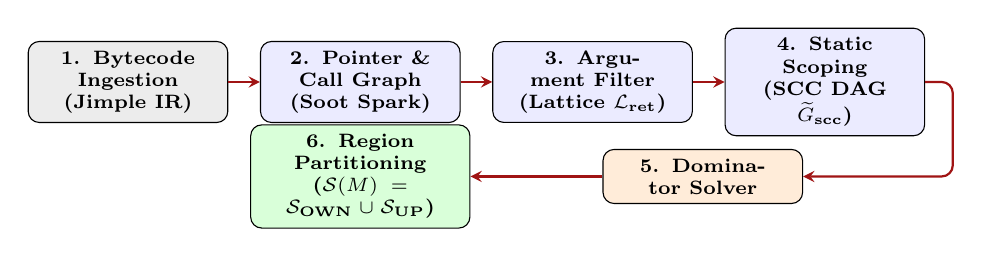
\begin{tikzpicture}[
    box/.style={draw, rectangle, rounded corners, fill=blue!8, text centered, minimum height=0.68cm, text width=2.30cm, font=\scriptsize\bfseries},
    arrow/.style={->, >=stealth, thick, darkred}
  ]
    \node[box, fill=gray!15] (ir) at (0.2,1.8) {1. Bytecode Ingestion\\(Jimple IR)};
    \node[box] (spark) at (3.15,1.8) {2. Pointer \& Call Graph\\(Soot Spark)};
    \node[box] (ret) at (6.1,1.8) {3. Argument Filter\\(Lattice $\mathcal{L}_{\text{ret}}$)};
    \node[box] (scoping) at (9.05,1.8) {4. Static Scoping\\(SCC DAG $\widetilde{G}_{\text{scc}}$)};

    \node[box, fill=orange!15] (csr) at (7.5,0.6) {5. Dominator Solver};
    \node[box, fill=green!15, text width=2.55cm] (part) at (3.15,0.6) {6. Region Partitioning\\($\mathcal{S}(M) = \mathcal{S}_{\text{OWN}} \cup \mathcal{S}_{\text{UP}}$)};

    \draw[arrow] (ir) -- (spark);
    \draw[arrow] (spark) -- (ret);
    \draw[arrow] (ret) -- (scoping);
    \draw[arrow, rounded corners=4pt] (scoping.east) -- ++(0.35,0) |- (csr.east);
    \draw[arrow] (csr) -- (part);
  \end{tikzpicture}
  \end{center}

  \begin{columns}[T]
    \begin{column}{0.48\textwidth}
      \begin{block}{Input: Unmodified Bytecode}
        \scriptsize
        \begin{itemize}\setlength{\itemsep}{1pt}
          \item Operates ahead-of-time on standard JVM \texttt{.class} files without source annotations.
          \item Whole-program analysis across application classes and runtime libraries.
        \end{itemize}
      \end{block}
    \end{column}
    \begin{column}{0.48\textwidth}
      \begin{block}{Output: Deterministic Partitions}
        \scriptsize
        \begin{itemize}\setlength{\itemsep}{1pt}
          \item Emits allocation partitions $\mathcal{P}(M)$ with deallocation bound to frame exits.
          \item Retains uncaptured objects in residual global heap $\mathcal{H}_{\text{GLOBAL}}$.
        \end{itemize}
      \end{block}
    \end{column}
  \end{columns}
\end{frame}
\endgroup

% ==============================================================================
% SECTION 2: DYNAMIC OWNERSHIP TREES & SEMANTIC FOUNDATIONS
% ==============================================================================
\section[Dynamic Ownership Trees]{Dynamic Ownership Trees \& Semantic Foundations}

\begin{frame}{Conceptual Shift: Escape vs. Heap Dominance}
  \begin{itemize}
    \item \textbf{Core Insight:} Object ownership is not a syntactic type: it is \textbf{topological graph dominance} over the execution call stack.
  \end{itemize}

  \begin{center}
    \footnotesize
    \begin{tabular}{>{\raggedright\arraybackslash}p{0.46\textwidth}>{\raggedright\arraybackslash}p{0.46\textwidth}}
      \toprule
      \textbf{Traditional Escape Analysis} & \textbf{Static Dominance Inference (DOSA)} \\
      \midrule
      \textbf{Question:} Does object $o$ escape method $m$? & \textbf{Question:} Which method frame is the unique topological dominator of object $o$? \\
      \addlinespace[2pt]
      \textbf{Output:} Binary classification ($\text{Escape} / \text{NoEscape}$). & \textbf{Output:} Exact capturing method frame $M$ and topological depth $k$. \\
      \addlinespace[2pt]
      \textbf{Action:} If $o$ escapes $m$, allocate in shared heap. & \textbf{Action:} Allocate $o$ in region $\mathcal{P}(M)$; reclaim at $M$ return. \\
      \bottomrule
    \end{tabular}
  \end{center}
  \vspace{-0.5em}

  \begin{block}{Execution State Formulation ($H_t$)}
    \footnotesize
    Call frames chain synchronously: $f_1 \to \dots \to f_n$ per thread. Augmented roots include static memory and concurrent threads: $\text{ROOT} \to \text{GLOBAL}$ and $\text{ROOT} \to \text{Thread}_i \to f_1^{(i)}$.
  \end{block}
\end{frame}

\begingroup
\setbeamerfont{block title}{size=\scriptsize}
\setbeamerfont{block title alerted}{size=\scriptsize}
\begin{frame}{Abstract Ownership Graph $G^\sharp$: Node Topologies}
  \vspace{-0.4em}
  {\scriptsize\textbf{Nodes:} $V^\sharp = \{\ROOT, \GLOBAL\} \cup \mathcal{M} \cup \mathcal{S} \cup \mathcal{U}_{\text{unsafe}}$ bounds all concrete execution states $H_t$.}\\[2pt]

  \begin{columns}[c]
    \begin{column}{0.28\textwidth}
      \centering
      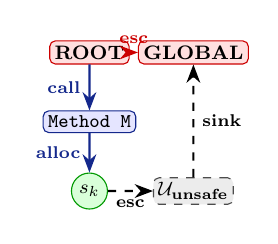
\begin{tikzpicture}[
        scale=0.88, every node/.style={transform shape},
        >=Stealth,
        root/.style={draw=red!80!black, fill=red!12, rounded corners=2pt, font=\footnotesize\bfseries, inner sep=2pt},
        frame/.style={draw=darkblue, fill=blue!10, rounded corners=2pt, font=\footnotesize\bfseries, inner sep=2pt},
        site/.style={draw=green!60!black, fill=green!15, circle, font=\footnotesize\bfseries, inner sep=1.8pt},
        sink/.style={draw=black!70, dashed, fill=gray!15, rounded corners=2pt, font=\footnotesize\bfseries, inner sep=2pt}
      ]
        \node[root]  (r) at (0.0, 2.7) {$\ROOT$};
        \node[root]  (g) at (1.5, 2.7) {$\GLOBAL$};
        \node[frame] (m) at (0.0, 1.7) {\texttt{Method M}};
        \node[site]  (s) at (0.0, 0.7) {$s_k$};
        \node[sink]  (u) at (1.5, 0.7) {$\mathcal{U}_{\text{unsafe}}$};

        \draw[->, thick, red!80!black] (r) -- node[above, font=\scriptsize\bfseries] {esc} (g);
        \draw[->, thick, darkblue]     (r) -- node[left, font=\scriptsize\bfseries] {call} (m);
        \draw[->, thick, darkblue]     (m) -- node[left, font=\scriptsize\bfseries] {alloc} (s);
        \draw[->, dashed, thick]       (s) -- node[below, font=\scriptsize\bfseries] {esc} (u);
        \draw[->, dashed, thick]       (u) -- node[right, font=\scriptsize\bfseries] {sink} (g);
      \end{tikzpicture}
    \end{column}

    \begin{column}{0.70\textwidth}
      \begin{block}{Node Universe Taxonomy ($V^\sharp$)}
        \scriptsize
        \begin{itemize}\setlength{\itemsep}{1.1pt}\setlength{\topsep}{0pt}\setlength{\partopsep}{0pt}\setlength{\parskip}{0pt}\setlength{\parsep}{0pt}
          \item \textbf{Sentinel Roots} ($\ROOT$: 0, $\GLOBAL$: 1): Universal entry and escaping sink. Nodes dominated by $\ROOT/\GLOBAL$ fall back safely to tracing GC.
          \item \textbf{Method Frame Nodes} ($\mathcal{M}$): Stack frames in $G_{\text{cg}}$ (IDs $2 \dots 1+|\mathcal{M}|$). Subtree roots in $T^\sharp$, governing private arenas $\mathcal{P}(M) = \text{Dead}(M)$.
          \item \textbf{Allocation Site Nodes} ($\mathcal{S}$): Bytecode \texttt{new} sites (IDs $\text{base} \dots$). Dominated leaves in $T^\sharp$ with lifetimes bounded by $\idom(s)$.
          \item \textbf{Unsafe Sinks} ($\mathcal{U}_{\text{unsafe}}$): Sinks for \texttt{Unsafe}/JNI. Retains escape cause; directs unconfined objects safely to $\GLOBAL \implies \mathcal{H}_{\GLOBAL}$.
        \end{itemize}
      \end{block}
    \end{column}
  \end{columns}
  \vspace{-0.5em}
  \begin{alertblock}{Dominator Graph Mapping: $G^\sharp \to T^\sharp = \dom(G^\sharp)$}
    \scriptsize
    In computed dominator tree $T^\sharp$, methods $\mathcal{M}$ become subtree roots governing private arenas $\mathcal{A}_M$, while allocation sites $\mathcal{S}$ become dominated leaves. Any site dominated by $\ROOT$ or $\GLOBAL$ defaults safely to $\mathcal{H}_{\GLOBAL}$.
  \end{alertblock}
\end{frame}
\endgroup

\begingroup
\setbeamerfont{block title}{size=\scriptsize}
\setbeamerfont{block title alerted}{size=\scriptsize}
\begin{frame}{Abstract Ownership Graph $G^\sharp$: Edge \& Dominator Semantics}
  \vspace{-0.6em}
  {\scriptsize\textbf{Dual-Stage Bounding:} Rules insert provenance edges; solver strips labels for CSR dominators $T^\sharp = \dom(G^\sharp)$.}\par\vspace{1pt}

  \begin{columns}[T,onlytextwidth]
    % Left Column: Edge Insertion Semantics
    \begin{column}{0.51\textwidth}
      \begin{block}{1. Ownership Graph Edge Rules ($E^\sharp$)}
        \fontsize{5.7pt}{6.8pt}\selectfont
        \setlength{\tabcolsep}{2.5pt}
        \begin{tabular}{@{}ll@{}}
          \toprule
          \textbf{Category} & \textbf{Edge Insertion Rule} \\
          \midrule
          \textbf{Call \& Root}    & $\ROOT \to \GLOBAL$, \quad $\ROOT \to m_{\text{entry}}$ \\
                                   & $\ROOT \to m_{\text{async}}$ \ (concurrency severing) \\
                                   & $m \to m'$ \ (synchronous call) \\
          \midrule
          \textbf{Heap \& Statics} & $s_1 \to s_2$ \ ($\forall s_2 \in \text{PointsTo}(s_1.f)$) \\
                                   & $\text{Scope}(F) \to s$ \ ($s \in \text{PointsTo}(F)$) \\
                                   & $\GLOBAL \to s$ \ (special sink / unconfined) \\
          \midrule
          \textbf{Frame Alloc}     & $m \to s$ \ ($x = \text{new } C, \ s = \text{AllocSite}$) \\
                                   & $m \to s$ \ ($x = y.p(\vec{z}) \land \top \in \retParams(p)$) \\
                                   & $\top \notin \retParams(p) \implies \text{Suppressed (Filter)}$ \\
          \bottomrule
        \end{tabular}
      \end{block}
    \end{column}

    % Right Column: Dominator Edges & Partitioning
    \begin{column}{0.47\textwidth}
      \begin{block}{2. Dominator Tree Edges ($T^\sharp = \dom(G^\sharp)$)}
        \fontsize{5.8pt}{7.0pt}\selectfont
        \begin{itemize}\setlength{\itemsep}{0.6pt}\setlength{\topsep}{0pt}\setlength{\parskip}{0pt}\setlength{\parsep}{0pt}
          \item \textbf{Dominance Criterion:}
            $d \dom n \iff$ all paths $\ROOT \rightsquigarrow n$ pass through $d$.
          \item \textbf{Immediate Dominator Edge:}
            $u \xrightarrow{\idom} v \iff u = \idom(v) \text{ in } T^\sharp$.
          \item \textbf{Single-Source Tree:} $T^\sharp$ rooted at $\ROOT$; unique parent $\idom(v)$.
        \end{itemize}
      \end{block}
      \vspace{-0.6em}
      \begin{alertblock}{3. Dominator Region Partitioning ($\idom \implies \mathcal{P}$)}
        \fontsize{5.7pt}{6.8pt}\selectfont
        \setlength{\tabcolsep}{2.5pt}
        \begin{tabular}{@{}ll@{}}
          \toprule
          \textbf{Dominator $\idom(s)$} & \textbf{Region Partition \& Safety} \\
          \midrule
          $\text{AllocMethod}(s)$ & $\mathbf{OWN}$: private method arena \\
          $\text{Ancestor Caller}$ & $\mathbf{UP}_k$: $k$-caller region arena \\
          $\{\ROOT, \GLOBAL\}$ & $\mathbf{HEAP}$: tracing GC fallback \\
          \bottomrule
        \end{tabular}\par\vspace{1pt}
        \textbf{Soundness Invariant:}
        $M = \idom_{G^\sharp}(s) \implies f_M^{\text{oldest}} \dom_{H_t} o$.
      \end{alertblock}
    \end{column}
  \end{columns}
\end{frame}
\endgroup

\begin{frame}[fragile]{Sub-Second CSR Dominator Solver}
  \vspace{-0.3em}
  \begin{itemize}\setlength{\itemsep}{1pt}
    \item \textbf{Topological Dominance on Large Graphs:} Whole-program graphs exceed $10^7$ edges; requires cache-local primitives.
  \end{itemize}
  \vspace{-0.4em}

  \begin{columns}[T]
    \begin{column}{0.48\textwidth}
      \begin{block}{1. CSR Graph Representation}
        \scriptsize
        \begin{itemize}\setlength{\itemsep}{1.5pt}
          \item \textbf{Forward CSR:} Flattened primitive \texttt{int[]} arrays: \texttt{offsets} ($|V|+1$) and \texttt{adjacency} ($|E|$).
          \item \textbf{Predecessor CSR:} Computes linear transpose (\texttt{poff}, \texttt{padj}) in $\mathcal{O}(|V| + |E|)$ time without object allocation.
          \item \textbf{Hardware Locality:} Eliminates pointer chasing; entire traversal executes within CPU L2/L3 cache.
          \item \textbf{Soundness Witness:} \texttt{dominates()} tests reachability; \texttt{witness()} extracts explicit paths bypassing candidate $d$.
        \end{itemize}
      \end{block}
    \end{column}

    \begin{column}{0.49\textwidth}
      \begin{block}{2. Cooper-Harvey-Kennedy Solver}
        \scriptsize
        \begin{itemize}\setlength{\itemsep}{1.5pt}
          \item \textbf{RPO Traversal:} Explicit DFS assigns post-order numbers; RPO order ensures 2--3 pass convergence.
          \item \textbf{Two-Finger Intersect:} Computes $\text{idom}(v) = \bigcap_{p} \text{idom}(p)$ via post-order finger climbing:
        \end{itemize}
        \vspace{-0.3em}
\begin{lstlisting}[style=javacodetiny, basicstyle=\fontsize{5.2pt}{6.2pt}\ttfamily]
while (f1 != f2) {
  while (postOrder[f1] < postOrder[f2]) f1 = idom[f1];
  while (postOrder[f2] < postOrder[f1]) f2 = idom[f2];
}
\end{lstlisting}
        \vspace{-0.6em}
        \begin{itemize}\setlength{\itemsep}{1.5pt}
          \item \textbf{Sub-Second Runtime:} 0.70s on \texttt{fop} (16.9M edges); $<2.5$s maximum across DaCapo.
        \end{itemize}
      \end{block}
    \end{column}
  \end{columns}
\end{frame}

\begingroup
\setbeamerfont{block title}{size=\scriptsize}
\begin{frame}[fragile]{Dynamic Ownership Trees \& Subtree Reclamation}
  \begin{itemize}
    \small
    \item \textbf{Theorem 4.3 (Subtree Reclamation):} When frame $f_n$ returns, all objects in $\text{Dead}(f_n) = \{ o \mid \text{idom}^*(o) = f_n \}$ are reclaimed in $\mathcal{O}(1)$ time.
  \end{itemize}
  \vspace{-0.6em}

  \begin{columns}[T,onlytextwidth]
    % Left Column: Verification Code & Table
    \begin{column}{0.47\textwidth}
      {\scriptsize\bfseries\color{darkblue} Verification Suite (\texttt{O01}): Local Frame Tree}\\[1pt]
\begin{lstlisting}[style=javacodetiny]
class Cache { static Box shared; }
void main() {
  Cache.shared = new Box(); // s1
  Box a = new Box();        // s2
  a.item = new Item();      // s3
  work();
}
void work() {
  Item b = new Item();      // s4
} // Dead(work) = {s4} reclaimed!
\end{lstlisting}
      \vspace{-0.6em}

      \begin{block}{Region Partitions \& Safety}
        \scriptsize
        \begin{tabular}{@{}ll@{}}
          \toprule
          \textbf{Site \& Target} & \textbf{Lifetime Guarantee} \\
          \midrule
          $s_4 \in \mathcal{P}(\texttt{work})$ & Bulk-reclaimed at $f_2$ exit \\
          $s_2, s_3 \in \mathcal{P}(\texttt{main})$ & Survives $f_2$ exit \\
          $s_1 \in \mathcal{H}_{\text{GLOBAL}}$ & Thread-shared static \\
          \bottomrule
        \end{tabular}
      \end{block}
    \end{column}

    % Right Column: Big, clear Ownership Tree
    \begin{column}{0.52\textwidth}
      \centering
      \vspace{-0.2em}
      {\footnotesize\bfseries Concrete Ownership Tree $T_t = \text{dom}(H_t)$}\\[1pt]
      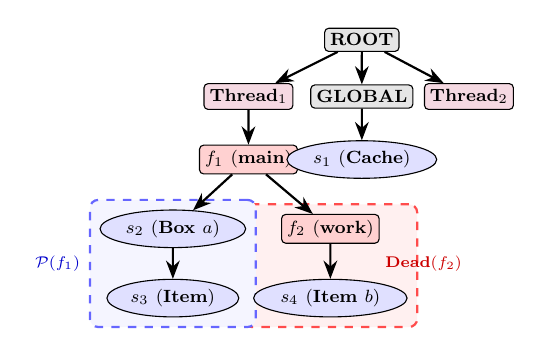
\begin{tikzpicture}[
        scale=0.80, every node/.style={transform shape},
        >=Stealth,
        sentinel/.style={draw, rectangle, rounded corners=1.5pt, fill=gray!20, font=\footnotesize\bfseries, inner sep=2.5pt},
        thread/.style={draw, rectangle, rounded corners=1.5pt, fill=purple!15, font=\footnotesize\bfseries, inner sep=2.5pt},
        frame/.style={draw, rectangle, rounded corners=1.5pt, fill=red!18, font=\footnotesize\bfseries, inner sep=2.5pt},
        obj/.style={draw, ellipse, fill=blue!12, font=\footnotesize\bfseries, inner sep=2pt}
      ]
        % Level 0: ROOT
        \node[sentinel] (root) at (3.1, 4.8) {$\text{ROOT}$};

        % Level 1: Augmented Roots
        \node[thread]   (t1)   at (1.3, 3.9) {$\text{Thread}_1$};
        \node[sentinel] (glob) at (3.1, 3.9) {$\text{GLOBAL}$};
        \node[thread]   (t2)   at (4.8, 3.9) {$\text{Thread}_2$};

        % Level 2: Under Thread 1 (main) and GLOBAL
        \node[frame] (f1) at (1.3, 2.9) {$f_1\ (\text{main})$};
        \node[obj]   (s1) at (3.1, 2.9) {$s_1\ (\text{Cache})$};

        % Level 3: Under f1 (captured s2, and callee f2)
        \node[obj]   (s2) at (0.1, 1.8) {$s_2\ (\text{Box } a)$};
        \node[frame] (f2) at (2.6, 1.8) {$f_2\ (\text{work})$};

        % Level 4: Under s2 (s3) and under f2 (s4)
        \node[obj]   (s3) at (0.1, 0.7) {$s_3\ (\text{Item})$};
        \node[obj]   (s4) at (2.6, 0.7) {$s_4\ (\text{Item } b)$};

        % Edges
        \draw[->, thick] (root) -- (t1);
        \draw[->, thick] (root) -- (glob);
        \draw[->, thick] (root) -- (t2);

        \draw[->, thick] (t1)   -- (f1);
        \draw[->, thick] (glob) -- (s1);

        \draw[->, thick] (f1) -- (s2);
        \draw[->, thick] (f1) -- (f2);

        \draw[->, thick] (s2) -- (s3);
        \draw[->, thick] (f2) -- (s4);

        % Dashed bounding box for Dead(work) = {s4}
        \begin{scope}[on background layer]
          \node[draw=red!70, dashed, thick, fill=red!6, rounded corners=3pt, fit=(f2) (s4), inner sep=3.5pt] (deadf2) {};
          \node[draw=blue!60, dashed, thick, fill=blue!4, rounded corners=3pt, fit=(s2) (s3), inner sep=3.5pt] (ownf1) {};
        \end{scope}
        \node[font=\scriptsize\bfseries, text=red!80!black, anchor=west] at (3.35, 1.25) {$\text{Dead}(f_2)$};
        \node[font=\scriptsize\bfseries, text=blue!80!black, anchor=east] at (-1.25, 1.25) {$\mathcal{P}(f_1)$};
      \end{tikzpicture}
    \end{column}
  \end{columns}
\end{frame}
\endgroup

\begingroup
\setbeamerfont{block title}{size=\scriptsize}
\begin{frame}[fragile]{Example: Container Stealing \& Move-Out}
  \begin{itemize}
    \small
    \item \textbf{Container Mutation \& Move-Out:} Callee populates caller container; caller moves element out.
  \end{itemize}
  \vspace{-0.85em}

  \begin{columns}[T,onlytextwidth]
    % Left Column: Verification Code & Classification
    \begin{column}{0.47\textwidth}
      {\fontsize{7.0pt}{8.2pt}\selectfont\bfseries\color{darkblue} Verification Suite (\texttt{O04}): Container Move-Out}\\[1pt]
\begin{lstlisting}[style=javacodetiny]
class Box { Item item; }
static void fill(Box b) {
  b.item = new Item(); // s_item
}
static Item take(Box b) {
  Item t = b.item; b.item = null; return t;
}
public static void main(String[] args) {
  Box box = new Box(); fill(box); // s_box
  Item moved = take(box);
} // Both die in main!
\end{lstlisting}
      \vspace{-0.8em}

      \begin{block}{Region Partitions \& Safety}
        \scriptsize
        \begin{tabular}{@{}ll@{}}
          \toprule
          \textbf{Site \& Region} & \textbf{Lifetime Guarantee} \\
          \midrule
          $s_{\text{box}} \in \mathcal{P}(\texttt{main})$ & $\mathbf{OWN}$: dies at \texttt{main} exit \\
          $s_{\text{item}} \in \mathcal{P}(\texttt{main})$ & $\mathbf{UP}_1$: dies at \texttt{main} exit \\
          \bottomrule
        \end{tabular}
      \end{block}
    \end{column}

    % Right Column: Unified Graphs inside ONE TikZ environment
    \begin{column}{0.51\textwidth}
      \vspace{-0.3em}
      \centering
      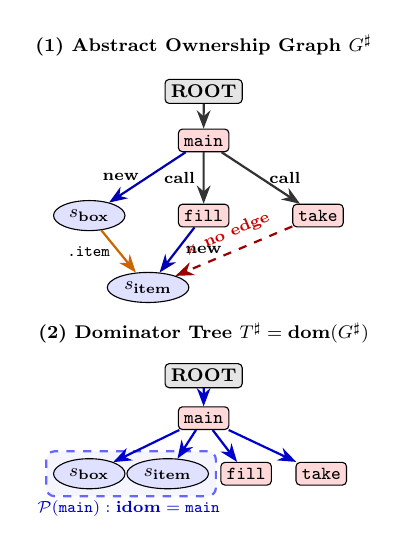
\begin{tikzpicture}[
        scale=0.83, every node/.style={transform shape},
        >=Stealth,
        sentinel/.style={draw, rectangle, rounded corners=1.5pt, fill=gray!20, font=\footnotesize\bfseries, inner sep=2.5pt},
        frame/.style={draw, rectangle, rounded corners=1.5pt, fill=red!15, font=\footnotesize\bfseries, inner sep=2.5pt},
        obj/.style={draw, ellipse, fill=blue!12, font=\footnotesize\bfseries, inner sep=2.2pt},
        call/.style={->, thick, draw=black!80},
        alloc/.style={->, thick, draw=blue!70!black},
        field/.style={->, thick, draw=orange!80!black},
        dom/.style={->, thick, draw=blue!80!black}
      ]
        % Title 1
        \node[font=\footnotesize\bfseries, text=black] at (2.0, 4.65) {(1) Abstract Ownership Graph $G^\sharp$};

        % G# nodes
        \node[sentinel] (root) at (2.0, 3.95) {$\text{ROOT}$};
        \node[frame]    (main) at (2.0, 3.20) {$\texttt{main}$};

        \node[obj]   (sbox) at (0.25, 2.05) {$s_{\text{box}}$};
        \node[frame] (fill) at (2.0,  2.05) {$\texttt{fill}$};
        \node[frame] (take) at (3.75, 2.05) {$\texttt{take}$};

        \node[obj]   (sitem) at (1.15, 0.95) {$s_{\text{item}}$};

        % G# edges
        \draw[call] (root) -- (main);
        \draw[alloc] (main) -- node[left, font=\scriptsize\bfseries] {new} (sbox);
        \draw[call] (main) -- node[left, font=\scriptsize\bfseries] {call} (fill);
        \draw[call] (main) -- node[right, font=\scriptsize\bfseries] {call} (take);

        \draw[field] (sbox) -- node[left, font=\scriptsize\bfseries] {\texttt{.item}} (sitem);
        \draw[alloc] (fill) -- node[right, font=\scriptsize\bfseries] {new} (sitem);

        \draw[->, thick, dashed, draw=red!60!black] (take) -- node[above=1pt, sloped, font=\scriptsize\bfseries, text=red!80!black] {$\times$ no edge} (sitem);

        % Title 2
        \node[font=\footnotesize\bfseries, text=black] at (2.0, 0.25) {(2) Dominator Tree $T^\sharp = \text{dom}(G^\sharp)$};

        % T# nodes
        \node[sentinel] (r) at (2.0, -0.40) {$\text{ROOT}$};
        \node[frame]    (m) at (2.0, -1.05) {$\texttt{main}$};

        \node[obj]   (b) at (0.25, -1.90) {$s_{\text{box}}$};
        \node[obj]   (i) at (1.45, -1.90) {$s_{\text{item}}$};
        \node[frame] (f) at (2.65, -1.90) {$\texttt{fill}$};
        \node[frame] (t) at (3.80, -1.90) {$\texttt{take}$};

        \draw[dom] (r) -- (m);
        \draw[dom] (m) -- (b);
        \draw[dom] (m) -- (i);
        \draw[dom] (m) -- (f);
        \draw[dom] (m) -- (t);

        \begin{scope}[on background layer]
          \node[draw=blue!60, dashed, thick, fill=blue!4, rounded corners=3pt, fit=(b) (i), inner sep=2.5pt] (dombox) {};
        \end{scope}
        \node[font=\scriptsize\bfseries, text=blue!80!black, anchor=north] at (0.85, -2.18) {$\mathcal{P}(\texttt{main}): \text{idom} = \texttt{main}$};
      \end{tikzpicture}
    \end{column}
  \end{columns}
\end{frame}
\endgroup

\begingroup
\setbeamerfont{block title}{size=\scriptsize}
\setbeamerfont{block title alerted}{size=\scriptsize}
\begin{frame}{The Argument-Passthrough Filter Algorithm}
  \vspace{-0.4em}
  {\scriptsize\textbf{Constructor Collapse Problem:} Returning \texttt{this} creates spurious cycles ($M \rightleftarrows C$), collapsing dominators to $\text{SUPER\_ROOT}$.}\\[2pt]

  \begin{columns}[T,onlytextwidth]
    \begin{column}{0.48\textwidth}
      \begin{block}{1. 64-Bit Param Lattice $\mathcal{L}_{\text{ret}}$}
        \scriptsize
        $\mathcal{L}_{\text{ret}} = \langle \mathcal{P}(\{\text{this}, p_1, \dots, p_{61}\}) \cup \{\top\}, \sqsubseteq \rangle$
        \begin{itemize}\setlength{\itemsep}{0.8pt}\setlength{\topsep}{0pt}\setlength{\partopsep}{0pt}\setlength{\parskip}{0pt}\setlength{\parsep}{0pt}
          \item \textbf{Bit 0:} \texttt{this} \quad \textbf{Bit $k$:} Param $p_k$ ($1\text{L} \ll k$)
          \item \textbf{Bit 63:} $\top$ (fresh allocation / global escape)
          \item \textbf{Join:} Bitwise OR ($\sqcup$) enables $\mathcal{O}(1)$ lattice join
        \end{itemize}
      \end{block}
      \vspace{-0.3em}
      \begin{center}
      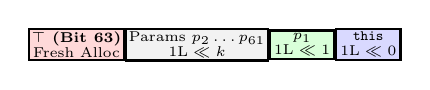
\begin{tikzpicture}[
        scale=0.86, every node/.style={transform shape},
        bitbox/.style={draw, thick, minimum height=0.40cm, font=\fontsize{5.8pt}{6.8pt}\selectfont, align=center, inner sep=1.2pt}
      ]
        \node[bitbox, fill=red!15, minimum width=1.35cm] (b63) at (0,0) {\textbf{$\top$ (Bit 63)}\\[-0.5pt]Fresh Alloc};
        \node[bitbox, fill=gray!10, minimum width=1.65cm, right=0pt of b63] (mid) {Params $p_2 \dots p_{61}$\\[-0.5pt]$1\text{L} \ll k$};
        \node[bitbox, fill=green!15, minimum width=0.95cm, right=0pt of mid] (b1) {\textbf{$p_1$}\\[-0.5pt]$1\text{L} \ll 1$};
        \node[bitbox, fill=blue!15, minimum width=0.95cm, right=0pt of b1] (b0) {\textbf{\texttt{this}}\\[-0.5pt]$1\text{L} \ll 0$};
      \end{tikzpicture}
      \end{center}
    \end{column}

    \begin{column}{0.50\textwidth}
      \begin{block}{2. Monotone Fixed-Point Solver}
        \scriptsize
        \begin{itemize}\setlength{\itemsep}{0.8pt}\setlength{\topsep}{0pt}\setlength{\partopsep}{0pt}\setlength{\parskip}{0pt}\setlength{\parsep}{0pt}
          \item \textbf{Forward RPO:} Propagates bitmasks on Jimple CFG.
          \item \textbf{Transfer Functions:}
            \vspace{1pt}
            \begin{tabular}{@{}ll@{}}
              $x = y \,|\, y.f$ & $\implies D_{\text{out}}[x] = D_{\text{in}}[y]$ \\
              $x = \text{new } C$ & $\implies D_{\text{out}}[x] = \top$ (Bit 63) \\
              $x = y.p(\vec{z})$ & $\implies$ Callee $\retParams[p]$
            \end{tabular}
          \item \textbf{Summary:} $\retParams(m) = \bigsqcup_{u \in \text{ret}(m)} D_{\text{out}}[u][r]$
          \item \textbf{Worklist:} Iterates over $G_{\text{cg}}$ until convergence.
        \end{itemize}
      \end{block}
    \end{column}
  \end{columns}
  \vspace{-0.5em}
  \begin{alertblock}{3. Dominance Preservation Rule (Frame-Call)}
    \scriptsize
    If $\top \notin \retParams(p)$, callee returns only caller arguments $\implies$ Suppress return edge $m \to s \in E^\sharp$ from Ownership Graph. Eliminates spurious cycles and preserves caller frame dominance.
  \end{alertblock}
\end{frame}
\endgroup

\begingroup
\setbeamerfont{block title}{size=\scriptsize}
\begin{frame}[fragile]{Example: The Argument-Passthrough Filter}
  \vspace{-0.3em}
  \begin{itemize}\setlength{\itemsep}{0pt}\setlength{\parskip}{0pt}
    \item \textbf{Receiver Return in Action:} Callee returns \texttt{this}; the passthrough filter identifies parameter 0 reuse and preserves caller frame dominance.
  \end{itemize}
  \vspace{-0.4em}

  \begin{columns}[T,onlytextwidth]
    \begin{column}{0.48\textwidth}
      {\scriptsize\bfseries\color{darkblue} Verification Suite (\texttt{O03}): Receiver Return (\texttt{return this})}\\[2pt]
\begin{lstlisting}[style=javacodetiny, basicstyle=\fontsize{6.2pt}{7.6pt}\selectfont\ttfamily]
public class FluentBuilder {
  private Item item;
  public FluentBuilder withItem(Item i) {
    this.item = i;
    return this; // Parameter 0 passthrough
  }
  public static void runPipeline() {
    Item it = new Item();
    FluentBuilder b = new FluentBuilder();
    b.withItem(it);
  } // Both objects die safely here!
}
\end{lstlisting}
    \end{column}

    \begin{column}{0.50\textwidth}
      {\scriptsize\bfseries\color{purple!90!black} Jimple IR: Parameter Passthrough}\\[2pt]
\begin{lstlisting}[style=jimplecode, basicstyle=\fontsize{6.2pt}{7.6pt}\selectfont\ttfamily]
FluentBuilder this := @this: FluentBuilder;
Item item := @parameter0: Item;
this.<FluentBuilder: Item item> = item;
return this; // Parameter Passthrough!
\end{lstlisting}
      \vspace{-0.4em}
      \begin{block}{Filter Evaluation \& Region Decision}
        \fontsize{6.0pt}{7.2pt}\selectfont
        \begin{itemize}\setlength{\itemsep}{1pt}\setlength{\parskip}{0pt}\setlength{\parsep}{0pt}
          \item \textbf{Boundary Seed:} $D[\text{entry}][\text{this}] = \text{0x01}$, $D[\text{entry}][i] = \text{0x02}$.
          \item \textbf{Summary:} $\retParams[\texttt{withItem}] = \text{0x01}$ ($\text{Bit 63} = 0 \implies \top \notin \retParams$).
          \item \textbf{Dominance Outcome:} Suppresses return edge $\texttt{withItem} \to \texttt{runPipeline}$.
          \item \textbf{Result:} Both objects bounded to $\mathcal{P}(\texttt{runPipeline})$: $\mathbf{OWN}$ region.
        \end{itemize}
      \end{block}
    \end{column}
  \end{columns}
\end{frame}
\endgroup

% ==============================================================================
% SECTION 3: STATIC SCOPING & METHOD REGION PARTITIONING
% ==============================================================================
\section[Static Scoping \& Regions]{Static Scoping \& Method Region Partitioning}

\begin{frame}{Static Field Scoping via Lowest Common Ancestor}
  \begin{itemize}
    \item Static fields are conventionally treated as global roots ($\text{GLOBAL} \to \text{Heap}$).
    \item \textbf{Program Observation:} Real-world applications often use static fields for temporary buffers, scratchpads, or thread-local caches.
  \end{itemize}

  \begin{block}{Algorithm: Static Scoping on Call Graph SCC DAG ($\widetilde{G}_{\text{scc}}$)}
    \small
    \begin{enumerate}
      \item \textbf{Accessors:} $\text{Accessors}(F) = \text{Readers}(F) \cup \text{Writers}(F) \cup \text{ClinitCallers}(F)$.
      \item \textbf{Condensation:} Project accessors onto call graph SCC DAG $\widetilde{G}_{\text{scc}}$ with super-root.
      \item \textbf{Dominator LCA:} $C_{\text{lca}}(F) = \mathrm{LCA}_{\text{idom}}(\{ \text{sccOf}[m] \mid m \in \text{Accessors}(F) \})$.
      \item \textbf{Binding:} If $C_{\text{lca}} \notin \{\text{SUPER\_ROOT}\} \cup \mathcal{C}_{\text{entry}}$, bind $F$ to frame $M_{\text{cap}}(F) = \text{CanonicalEntryMethod}(C_{\text{lca}})$; otherwise falls back to $\text{GLOBAL}$.
    \end{enumerate}
  \end{block}
\end{frame}

\begingroup
\setbeamerfont{block title}{size=\scriptsize}
\begin{frame}[fragile]{Example: Cross-Frame Static Scoping}
  \begin{itemize}
    \small
    \item \textbf{Cross-Frame Static State:} Callee methods communicate through temporary static field \texttt{sess}, bounded by caller \texttt{runSession()}.
  \end{itemize}
  \vspace{-0.6em}

  \begin{columns}[T,onlytextwidth]
    \begin{column}{0.48\textwidth}
      {\scriptsize\bfseries\color{darkblue} Verification Suite (\texttt{O09}): Static Scoping}\\[1pt]
\begin{lstlisting}[style=javacodetiny, basicstyle=\fontsize{6.0pt}{7.4pt}\selectfont\ttfamily]
class BatchJobManager {
  static Session sess;
  public static void runSession(String c) {
    setup(c); // Writes static field
    work();   // Reads static field
    teardown(); // sess = null
  } // Arena reclaimed upon exit!
  static void setup(String c) { sess = new Session(c); }
  static void work()     { sess.run(); }
  static void teardown() { sess = null; }
}
\end{lstlisting}
      \vspace{-0.5em}

      \begin{block}{Static Scoping Resolution}
        \fontsize{6.4pt}{7.6pt}\selectfont
        \begin{tabular}{@{}ll@{}}
          \toprule
          \textbf{Analysis Step} & \textbf{Deduction} \\
          \midrule
          $\text{Accessors}(\texttt{sess})$ & $\{\texttt{setup}, \texttt{work}\}$ \\
          $\text{LCA}_{\text{idom}}$ in Call DAG & $\texttt{runSession}$ \\
          Capturing Frame & $M_{\text{cap}}(\texttt{sess}) = \texttt{runSession}$ \\
          Region Scope & $\mathcal{P}(\texttt{runSession})$ (frame exit) \\
          \bottomrule
        \end{tabular}
      \end{block}
    \end{column}

    \begin{column}{0.50\textwidth}
      \centering
      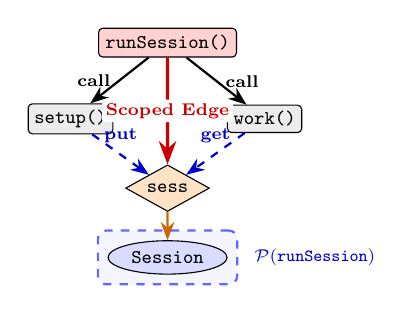
\begin{tikzpicture}[
        scale=0.88, every node/.style={transform shape},
        >=Stealth,
        ctrl/.style={draw, rectangle, rounded corners=1.5pt, fill=red!18, font=\footnotesize\bfseries, inner sep=2.8pt},
        callee/.style={draw, rectangle, rounded corners=1.5pt, fill=gray!15, font=\footnotesize\bfseries, inner sep=2.5pt},
        fld/.style={draw, diamond, aspect=1.8, fill=orange!22, font=\footnotesize\bfseries, inner sep=2.0pt},
        obj/.style={draw, ellipse, fill=blue!14, font=\footnotesize\bfseries, inner sep=2.4pt}
      ]
        \node[ctrl]   (c)  at (2.0, 3.1) {\texttt{runSession()}};
        \node[callee] (s1) at (0.6, 2.0) {\texttt{setup()}};
        \node[callee] (s2) at (3.4, 2.0) {\texttt{work()}};
        \node[fld]    (f)  at (2.0, 1.0) {\texttt{sess}};
        \node[obj]    (o)  at (2.0, 0.0) {\texttt{Session}};

        % Call edges
        \draw[->, thick] (c) -- node[left, font=\scriptsize\bfseries] {call} (s1);
        \draw[->, thick] (c) -- node[right, font=\scriptsize\bfseries] {call} (s2);

        % Accessor read/write edges
        \draw[->, dashed, thick, blue!80!black] (s1) -- node[above=1pt, font=\scriptsize\bfseries] {put} (f);
        \draw[->, dashed, thick, blue!80!black] (s2) -- node[above=1pt, font=\scriptsize\bfseries] {get} (f);

        % Scoped edge
        \draw[->, very thick, red!80!black] (c) -- node[fill=white, rounded corners=1pt, inner sep=1.5pt, font=\scriptsize\bfseries, text=red!80!black] {Scoped Edge} (f);
        \draw[->, thick, orange!80!black] (f) -- (o);

        % Region box enclosing allocated Session object
        \begin{scope}[on background layer]
          \node[draw=blue!60, dashed, thick, fill=blue!4, rounded corners=3pt, fit=(o), inner sep=3.5pt] (reg) {};
        \end{scope}
        \node[font=\scriptsize\bfseries, text=blue!80!black, anchor=west] at (reg.east) {\ $\mathcal{P}(\texttt{runSession})$};
      \end{tikzpicture}

      \vspace{0.1em}
      \begin{block}{Lemma 7.4: Static Scope Invariance}
        \fontsize{6.2pt}{7.4pt}\selectfont
        $\forall F \in \mathcal{F}_{\text{static}}$ where $M_{\text{cap}} \neq \text{null}$, an activation of $M_{\text{cap}}$ is active on stack during all accesses to $F$.
      \end{block}
    \end{column}
  \end{columns}
\end{frame}
\endgroup

\begingroup
\setbeamerfont{block title}{size=\scriptsize}
\begin{frame}[fragile]{Example: Condensation \& Super-Root ($\widetilde{G}_{\text{scc}}$)}
  \begin{columns}[T,onlytextwidth]
    \begin{column}{0.44\textwidth}
      {\scriptsize\bfseries\color{darkblue} Verification Suite (\texttt{O11}/\texttt{O12}): Threads \& Cycles}\\[2pt]
\begin{lstlisting}[style=javacodetiny]
class Job {
  static Metric metrics; // Multi-thread
  static Cache cache;    // Recursive
  void processBatch(int n) {
    metrics = new Metric();
    new Thread(new Log()).start(); // Async
    for (int i = 0; i < n; i++)
      format(i);
  }
  void format(int v) { helper(v); }
  void helper(int v) { format(v); } // Cycle
}
class Log implements Runnable {
  public void run() { Job.metrics.flush(); }
}
\end{lstlisting}
    \end{column}

    \begin{column}{0.55\textwidth}
      \centering
      \vspace{-0.2em}
      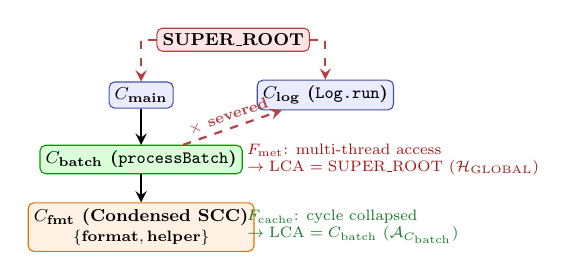
\begin{tikzpicture}[
        scale=0.78, every node/.style={transform shape},
        superroot/.style={rectangle, draw=darkred!80, fill=red!10, rounded corners=2pt, font=\footnotesize\bfseries, inner sep=2.6pt},
        scc/.style={rectangle, draw=darkblue!80, fill=blue!8, rounded corners=2pt, font=\footnotesize\bfseries, inner sep=2.6pt, align=center},
        scc_cond/.style={rectangle, draw=orange!90!black, fill=orange!10, rounded corners=2pt, font=\footnotesize\bfseries, inner sep=2.6pt, align=center},
        edge/.style={->, >=stealth, thick},
        async_edge/.style={->, >=stealth, thick, dashed, darkred!80},
        super_edge/.style={->, >=stealth, thick, dashed, darkred!80}
      ]
        \node[superroot] (SR) at (0, 3.2) {$\text{SUPER\_ROOT}$};
        \node[scc] (Cmain) at (-1.5, 2.3) {$C_{\text{main}}$};
        \node[scc] (Clog)  at (1.5, 2.3)  {$C_{\text{log}}$ (\texttt{Log.run})};
        \node[scc, fill=green!15, draw=green!60!black] (Cbatch) at (-1.5, 1.25) {$C_{\text{batch}}$ (\texttt{processBatch})};
        \node[scc_cond] (Cfmt) at (-1.5, 0.15) {$C_{\text{fmt}}$ (Condensed SCC)\\{\scriptsize $\{\text{format}, \text{helper}\}$}};

        % Edges from SUPER_ROOT
        \draw[super_edge] (SR) -| (Cmain);
        \draw[super_edge] (SR) -| (Clog);

        % Call edges
        \draw[edge] (Cmain) -- (Cbatch);
        \draw[edge] (Cbatch) -- (Cfmt);

        % Severed async edge
        \draw[async_edge] (Cbatch) -- node[above=-1pt, sloped, font=\scriptsize\bfseries] {$\times$ severed} (Clog);

        % Annotations on fields
        \node[align=left, font=\scriptsize, text=darkred, anchor=west] at (0.10, 1.25) {
          $F_{\text{met}}$: multi-thread access\\
          $\to \text{LCA} = \text{SUPER\_ROOT} \ (\mathcal{H}_{\text{GLOBAL}})$
        };
        \node[align=left, font=\scriptsize, text=darkgreen, anchor=west] at (0.10, 0.15) {
          $F_{\text{cache}}$: cycle collapsed\\
          $\to \text{LCA} = C_{\text{batch}} \ (\mathcal{A}_{C_{\text{batch}}})$
        };
      \end{tikzpicture}

      \vspace{-0.4em}
      \begin{block}{Why Both Steps Are Essential}
        \scriptsize
        \begin{itemize}\setlength{\itemsep}{1.5pt}\setlength{\parsep}{0pt}
          \item \textbf{Condensation ($G_{\text{scc}}$):} Mutual recursion cycles $\{\text{format}, \text{helper}\}$ collapse into a DAG node, making dominator trees well-defined.
          \item \textbf{Super-Root Concurrency Severing:} Severing async thread edges forces shared statics to $\text{SUPER\_ROOT}$ ($\mathcal{H}_{\text{GLOBAL}}$), preventing cross-thread use-after-free.
        \end{itemize}
      \end{block}
    \end{column}
  \end{columns}
\end{frame}
\endgroup

\begin{frame}[fragile]{Example: Safety Guard: Scope Lifting}
  \begin{itemize}
    \item \textbf{Soundness Hazard:} Static field retains state across consecutive calls (re-entrancy or lazy initialization).
  \end{itemize}

  \begin{columns}[T]
    \begin{column}{0.5\textwidth}
      {\scriptsize\bfseries\color{darkblue} Verification Suite (\texttt{O13}): Recurrent Static Cache}\\[2pt]
\begin{lstlisting}[style=javacodetiny]
public class Processor {
  private static Table table;
  public static void runBatch(int[] ids) {
    for (int id : ids) process(id);
  }
  public static void process(int id) {
    Table t = table; // Upward-exposed read
    if (t == null) table = new Table();
    table.query(id);
  }
}
\end{lstlisting}
    \end{column}
    \begin{column}{0.48\textwidth}
      \begin{alertblock}{Theorem 7.7: Boundary Re-Entrancy}
        \footnotesize
        If liveness detects an upward-exposed read without prior must-def:
        $$\text{LiveIn}(C_{\text{cand}}, F) = \text{true}$$
        Premature reclamation at $C_{\text{cand}}$ exit would cause an invalid recurrent access.
        \vspace{0.1em}
        
        \textbf{Action:} Iteratively lifts $C_{\text{cand}} \gets \text{idom}[C_{\text{cand}}]$ until reaching non-live-in ancestor or \textbf{HEAP}.
      \end{alertblock}
    \end{column}
  \end{columns}
\end{frame}

\begin{frame}{Method-Associated Memory Partitioning ($\mathcal{P}(M)$)}
  \vspace{-0.3em}
  \begin{itemize}
    \item Each method frame $M$ defines an independent memory partition:
      $$\mathcal{S}(M) = \mathcal{S}_{\text{OWN}}(M) \cup \bigcup_{k \ge 1} \mathcal{S}_{\text{UP}_k}(M), \qquad \mathcal{F}(M) = \mathcal{F}_{\text{static}}(M)$$
  \end{itemize}
  \vspace{-0.4em}
  \begin{block}{The Method Arena Runtime Model ($\mathcal{A}_M$)}
    \small
    \begin{itemize}\setlength{\itemsep}{1.5pt}
      \item \textbf{Prologue:} When method $M$ is entered, a thread-local arena $\mathcal{A}_M$ is instantiated.
      \item \textbf{Allocation:} Sites $s \in \mathcal{P}(M)$ use bump-pointer allocation ($ptr \gets ptr + size$).
      \item \textbf{Epilogue:} When $M$ returns, $\text{FreeRegion}(\mathcal{A}_M)$ bulk-reclaims all allocated pages in $\mathcal{O}(1)$ time without traversing object reference graphs.
      \item \textbf{Residual Heap:} $\mathcal{H}_{\text{GLOBAL}} = \mathcal{H} \setminus \biguplus_{M} \mathcal{P}(M)$ managed by traditional GC.
    \end{itemize}
  \end{block}
\end{frame}

% ==============================================================================
% SECTION 4: EMPIRICAL EVALUATION
% ==============================================================================
\section[Empirical Evaluation]{Empirical Evaluation}

\begin{frame}{Static Ownership Analysis Results (DaCapo 9.12-MR1)}
  \vspace{-0.4em}
  \begin{table}[h]
    \centering
    \scriptsize
    \setlength{\tabcolsep}{3.8pt}
    \renewcommand{\arraystretch}{1.12}
    \begin{tabular}{lrrrrrrr}
      \toprule
      \textbf{Metric} & \textbf{avrora} & \textbf{fop} & \textbf{h2} & \textbf{luindex} & \textbf{pmd} & \textbf{xalan} & \textbf{Total} \\
      \midrule
      App Alloc Sites & 1{,}005 & 6{,}373 & 1{,}625 & 910 & 899 & 206 & 11{,}018 \\
      \UP{} (Before Static Scoping) & 3 & 31 & 24 & 8 & 26 & 8 & 100 \\
      \UP{} (After Static Scoping) & 131 & 132 & 24 & 36 & 109 & 9 & 441 \\
      \UP{} Share of App Sites & 13.03\% & 2.07\% & 1.48\% & 3.96\% & 12.12\% & 4.37\% & 4.00\% \\
      \midrule
      Total Static Fields & 4{,}970 & 5{,}899 & 4{,}966 & 4{,}573 & 5{,}295 & 4{,}485 & 30{,}188 \\
      Scoped Static Fields & 574 & 801 & 424 & 249 & 375 & 126 & 2{,}549 \\
      Scoped Static Fields Share & 11.55\% & 13.58\% & 8.54\% & 5.45\% & 7.08\% & 2.81\% & 8.44\% \\
      \bottomrule
    \end{tabular}
  \end{table}

  \vspace{-0.2em}
  \begin{itemize}\setlength{\itemsep}{2pt}
    \item \textbf{Application Site Rescue:} Static Scoping reclassifies \textbf{341 application allocation sites} from \HEAP{} to method-scoped \UP{} regions ($100 \to 441$ sites).
    \item \textbf{Static Field Scoping:} Binds \textbf{2{,}549 static fields} (8.44\% across the suite) to controller method execution frames.
  \end{itemize}
\end{frame}

\begin{frame}{Whole-Program Partitioning \& Static Field Capture}
  \begin{columns}[T]
    \begin{column}{0.48\textwidth}
      \begin{block}{Whole-Program Metrics}
        \begin{itemize}
          \item \textbf{22,971 Sites Captured (28.0\% of 81,964 Total):}
            \begin{itemize}
              \item $\mathcal{S}_{\text{OWN}}$: 19,832 sites (86.3\% of captured)
              \item $\mathcal{S}_{\text{UP}}$: 3,139 sites (13.7\% of captured)
            \end{itemize}
          \item \textbf{11,119 Active Method Regions} formed across whole-program benchmarks.
          \item \textbf{2,549 Static Fields} bounded to method lifecycles.
        \end{itemize}
      \end{block}
    \end{column}
    \begin{column}{0.48\textwidth}
      \begin{alertblock}{Power-Law Static Distribution}
        Static field lifecycles are heavily concentrated:
        \begin{itemize}
          \item Just \textbf{18 super-controller methods} capture $>68\%$ (1,732 fields) of all scoped statics.
          \item Top controllers: \texttt{startFOP} (289 fields in \texttt{fop}), \texttt{Parser.parse} (162 fields in \texttt{h2}), and parser loops.
        \end{itemize}
      \end{alertblock}
    \end{column}
  \end{columns}
\end{frame}

\begingroup
\setbeamerfont{block title}{size=\scriptsize}
\begin{frame}{OpenJ9 Hardware Debug Counter Verification}
  \vspace{-0.5em}
  {\scriptsize\textbf{Physical Hardware Measurements:} Runtime verification on modified Eclipse OpenJ9 JDK 25:}\par\vspace{2pt}

  \begin{table}[h]
    \centering
    \scriptsize
    \setlength{\tabcolsep}{3.5pt}
    \renewcommand{\arraystretch}{1.18}
    \begin{tabular}{@{}lrr@{}}
      \toprule
      \textbf{Runtime Verification Metric} & \textbf{Standard OpenJ9} & \textbf{DOSA Arenas} \\
      \midrule
      Total Dynamic Allocation & 7,630.99 MB (2.07M evts) & 7,630.99 MB (2.07M evts) \\
      Dynamic Memory Churn Diverted & 0 MB (Nearly none) & \textbf{526.95 MB (Up to 49.30\%)} \\
      Inter-Procedural Region Objects & 0 (Nearly none; to GC) & \textbf{1,179,574 (29.29 MB)} \\
      Dynamic Objects Bypassing GC & 1,825 objs ($<$0.001\%) & \textbf{1,179,574 objs (29.29 MB)} \\
      \bottomrule
    \end{tabular}
  \end{table}

  \vspace{-0.3em}
  \begin{block}{Dynamic Memory Churn Impact}
    \scriptsize
    \begin{itemize}\setlength{\itemsep}{1.5pt}\setlength{\topsep}{0pt}\setlength{\parskip}{0pt}\setlength{\parsep}{0pt}
      \item \textbf{Total Dynamic Run Allocation:} \textbf{7,630.99 MB (7.63 GB)} across 2,070,081 allocation events. Standard OpenJ9 has nearly none of this optimization, routing all churn to tracing GC.
      \item \textbf{Unconstrained Dynamic Churn:} DOSA diverts \textbf{526.95 MB} into method arenas (366.96 MB in \texttt{h2}, 127.95 MB in \texttt{pmd}).
      \item \textbf{Churn Impact Share ($\lambda_{\text{arena}}$):} Diverts \textbf{6.51\%} baseline in \texttt{avrora}, surging to \textbf{49.30\%} with 3-round library inlining.
      \item \textbf{Dynamic Execution Footprint:} Analyzed 100\% of candidate sites (20,143 ingested); 746 sites were dynamically executed during benchmark runs (3.70\% active footprint), capturing all 1.18M objects.
    \end{itemize}
  \end{block}
\end{frame}
\endgroup

% ==============================================================================
% SECTION 5: JIT REALIZATION, DISCUSSION & CONCLUSION
% ==============================================================================
\section[Future Directions]{OpenJ9 JIT Realization \& Future Directions}

\begin{frame}{Direction 1: OpenJ9 Testarossa JIT Realization}
  \vspace{-0.5em}
  \begin{itemize}\setlength{\itemsep}{0pt}
    \item Moving from ahead-of-time bytecode tagging to physical JIT code emission:
  \end{itemize}
  \vspace{-0.6em}
  \begin{block}{JIT Compilation Pipeline Hooks}
    \small
    \begin{enumerate}\setlength{\itemsep}{0.5pt}
      \item \textbf{Prologue Injection:} Allocate a 64KB thread-local chunk on frame entry:
        \vspace{-0.3em}
        $$\texttt{TR::TreeTop} \longrightarrow \texttt{call vmHelper\_allocateArena}$$
        \vspace{-0.4em}
      \item \textbf{Fast-Path Bump Allocation:} Inlined JIT assembly replaces \texttt{new}:
        \vspace{-0.3em}
        $$\texttt{lea rax, [r15+size]}; \quad \texttt{cmp rax, r14}; \quad \texttt{mov [r15], rax}$$
        \vspace{-0.5em}
      \item \textbf{Atomic Epilogue Reset:} Reset arena pointer on return with zero GC book-keeping.
      \item \textbf{Write Barrier Elision:} Intra-arena stores never cross generations; elides post-store card marking (\texttt{CARD\_DIRTY}) to record old-to-young pointers, saving 2--4 cycles.
    \end{enumerate}
  \end{block}
\end{frame}

\begin{frame}{Direction 2: Adaptive Arena Profitability Heuristics}
  \begin{itemize}
    \item \textbf{The Trade-Off:} Instantiating arenas for all 11,119 active methods would introduce excessive prologue overhead for cold methods.
  \end{itemize}

  \begin{block}{Dual-Threshold Profitability Model}
    A method $M$ is selected for physical JIT arena compilation iff:
    $$W_{\text{dyn}}(M) \ge 1.0\text{ MB} \quad \land \quad \rho(M) \ge 1.0\text{ KB/invocation}$$
    \begin{itemize}
      \item Filters out short-lived leaf functions.
      \item Directs JIT code-bloat budget strictly toward high-churn batch controllers.
      \item Mitigates young-generation nursery churn and scavenge pauses.
    \end{itemize}
  \end{block}
\end{frame}

\begin{frame}{Direction 3: Dominator GC \& Bytecode Borrowing}
  \begin{columns}[T]
    \begin{column}{0.48\textwidth}
      \begin{block}{Dominator Tagging for GC}
        \small
        \begin{itemize}\setlength{\itemsep}{2pt}
          \item Encode static dominator depth into 2 bits of the object header.
          \item Allows GC scavenger to reclaim entire subgraphs in a single pass without recursive child tracing.
          \item Bypasses Cheney pointer forwarding ($T_{\text{evac}}$) and halts Tenured promotion ($R_{\text{promo}}^{\text{opt}} = 0$), avoiding Full GC compaction.
        \end{itemize}
      \end{block}
    \end{column}
    \begin{column}{0.48\textwidth}
      \begin{block}{Project Verona Isolated Regions}
        \small
        \begin{itemize}\setlength{\itemsep}{2pt}
          \item Formalize isolated subgraphs bounded by single-entry \emph{bridge objects}.
          \item Reclaim or migrate entire subgraphs in constant time upon bridge death or thread transfer.
          \item Enforce compile-time bytecode borrow contracts directly on Jimple IR.
        \end{itemize}
      \end{block}
    \end{column}
  \end{columns}
\end{frame}

\begin{frame}{Direction 4: Speculative Region Allocation \& Heapification}
  \begin{itemize}
    \item \textbf{Static Analysis Ceiling:} Pure ahead-of-time analysis conservatively demotes allocation sites to \HEAP{} upon unresolved virtual calls, dynamic reflection, or uncertain branches.
  \end{itemize}

  \begin{columns}[T]
    \begin{column}{0.48\textwidth}
      \begin{block}{CoSSJIT Speculative Invariants}
        \small
        Integrate with speculative compiler conditions:
        \begin{itemize}\setlength{\itemsep}{2pt}
          \item \textbf{SMC:} Speculative Method-Call (devirtualizes monomorphic call sites).
          \item \textbf{SMI:} Speculative Method-Inline.
          \item \textbf{SBE:} Speculative Branch-Execution (prunes cold exception edges).
        \end{itemize}
      \end{block}
    \end{column}
    \begin{column}{0.48\textwidth}
      \begin{alertblock}{Dynamic Heapification Fallback}
        \small
        \begin{itemize}\setlength{\itemsep}{2pt}
          \item Sites allocate speculatively within method arenas $\mathcal{A}_M$.
          \item If speculative check fails at runtime, OpenJ9 \emph{dynamic heapification} demotes objects to generational heap on demand.
          \item Preserves compiled JIT code execution without costly deoptimization.
        \end{itemize}
      \end{alertblock}
    \end{column}
  \end{columns}
\end{frame}

\begin{frame}{Conclusion \& Contributions}
  \begin{itemize}
    \item \textbf{Dominance-Based Formulation:} Formalized Dynamic Ownership Trees ($T_t$) to model method-scoped lifetimes via stack dominance.
    \item \textbf{Interprocedural Filtering:} Identified constructor-induced cyclic shortcuts ($G_N$) and introduced the Argument-Passthrough Filter ($\mathcal{L}_{\text{ret}}$).
    \item \textbf{Static Scoping:} Formulated Static Scoping on $\widetilde{G}_{\text{scc}}$, scoping 2,549 static fields and capturing 341 additional application sites across DaCapo.
    \item \textbf{Empirical Evaluation:} Demonstrated 22,971 captured sites (28.0\% of 81,964 whole-program sites), with OpenJ9 debug counters tracking 29.29 MB (1.18M objects) in candidate arenas.
  \end{itemize}

  \vspace{1em}
  \centering
  \Large \textbf{Thank You!} \\
  \vspace{0.5em}
  \small Questions \& Discussion
\end{frame}

% ==============================================================================
% APPENDIX
% ==============================================================================
\appendix
\section[Appendix]{Appendix}

\begin{frame}{Appendix: Handling Dynamic Reflection}
  \begin{itemize}
    \small
    \item \textbf{Dynamic Features in Java:} Reflection (\texttt{Class.newInstance}, \texttt{Method.invoke}) and dynamic loading cannot be resolved solely via ahead-of-time class hierarchy analysis.
  \end{itemize}
  \vspace{-0.4em}

  \begin{columns}[T]
    \begin{column}{0.48\textwidth}
      \begin{block}{Trace-Driven Call Resolution}
        \scriptsize
        \begin{itemize}\setlength{\itemsep}{2pt}
          \item \textbf{TamiFlex Profiler:} Logs concrete reflective target signatures during benchmark execution.
          \item \textbf{Call Graph Expansion:} Extends $G_{\text{cg}}$ with observed reflective targets during points-to analysis.
          \item \textbf{Resolution:} Captures regular method call patterns across profiled benchmark runs.
        \end{itemize}
      \end{block}
    \end{column}

    \begin{column}{0.48\textwidth}
      \begin{block}{Conservative Safety Fallback}
        \scriptsize
        \begin{itemize}\setlength{\itemsep}{2pt}
          \item \textbf{Lattice Default:} For unmodeled reflective targets, return lattice assigns $\top$:
            $$\mathcal{L}_{\text{ret}}(m_{\text{refl}}) = \top$$
          \item \textbf{Global Route:} Objects escape to $\text{GLOBAL}$ (\HEAP{}), preventing unsound stack or arena allocation.
          \item \textbf{Safety Invariant:} Unmodeled targets fail safe to tracing GC.
        \end{itemize}
      \end{block}
    \end{column}
  \end{columns}
\end{frame}

\begin{frame}{Appendix: Formal Soundness Metatheory}
  \small Complete formal soundness established through four inductive lemmas and four theorems:
  \vspace{0.1em}
  
  \begin{columns}[T]
    \begin{column}{0.48\textwidth}
      \begin{block}{Foundational Lemmas}
        \scriptsize
        \begin{itemize}\setlength{\itemsep}{1pt}
          \item \textbf{Lemma 7.1 (Path Preservation):} Concrete paths in $H_t$ are preserved in $G^\sharp$.
          \item \textbf{Lemma 7.2 (Call Chain Invariance):} Dominance in $G^\sharp$ guarantees stack dominance.
          \item \textbf{Lemma 7.3 (Thread Confinement):} Cross-thread publications sever to \texttt{GLOBAL}.
          \item \textbf{Lemma 7.4 (Static Scope Invariance):} $M_{\text{cap}}$ is active on stack during static access.
        \end{itemize}
      \end{block}
    \end{column}
    \begin{column}{0.48\textwidth}
      \begin{block}{Soundness Theorems}
        \scriptsize
        \begin{itemize}\setlength{\itemsep}{1pt}
          \item \textbf{Theorem 7.5 (Dominator Soundness):} Subtree reclamation preserves reference validity.
          \item \textbf{Theorem 7.6 (Residual Global Invariant):} Formalizes the 5 immortal escape predicates.
          \item \textbf{Theorem 7.7 (Boundary Re-Entrancy):} Live-in scope lifting prevents invalid accesses.
          \item \textbf{Theorem 7.8 (Frame Reclamation):} Dangling-pointer-free reclamation at frame exit.
        \end{itemize}
      \end{block}
    \end{column}
  \end{columns}
\end{frame}

\begin{frame}{Appendix: The 5 Immortal Escape Predicates (Theorem 7.6)}
  \footnotesize Theorem 7.6 (Residual Global Invariant) formalizes the 5 conditions requiring fallback to $\mathcal{H}_{\text{GLOBAL}}$:

  \vspace{-0.3em}
  \begin{table}[h]
    \centering
    \tiny
    \setlength{\tabcolsep}{3pt}
    \renewcommand{\arraystretch}{1.12}
    \begin{tabular}{@{}llp{5.4cm}@{}}
      \toprule
      \textbf{Predicate} & \textbf{Condition in $G^\sharp$} & \textbf{Safety Invariant \& Fallback Resolution} \\
      \midrule
      \textbf{P1: Concurrency} & $\text{idom}(o) = \text{SUPER\_ROOT}$ & Published across threads; thread lifecycles diverge asynchronously. \\
      \textbf{P2: Unbound Static} & $C_{\text{lca}}(F) \in \{\text{SUPER\_ROOT}\} \cup \mathcal{C}_{\text{entry}}$ & Static field accessible across entire program; cannot be method-scoped. \\
      \textbf{P3: Native (JNI)} & Passed to native method & Memory management outside JVM; cannot guarantee arena safety. \\
      \textbf{P4: Finalizers} & $\text{hasFinalizer}(o) = \text{true}$ & Finalizer outlives frame; requires standard GC finalization queue. \\
      \textbf{P5: Dynamic Refl.} & $\mathcal{L}_{\text{ret}}(m_{\text{refl}}) = \top$ & Unmodeled reflective call site; conservative fallback to tracing GC. \\
      \bottomrule
    \end{tabular}
  \end{table}

  \vspace{-0.5em}
  \begin{block}{Soundness Guarantee}
    \scriptsize
    Every object not satisfying any of P1--P5 is strictly dominated by an execution frame $M$, guaranteeing safe bulk reclamation at $M$ exit.
  \end{block}
\end{frame}

\begin{frame}{Appendix: Concurrency Boundary \& Thread Severing}
  \begin{itemize}
    \item When an object reference is published across concurrent threads, thread lifecycles diverge asynchronously.
  \end{itemize}

  \begin{columns}[T]
    \begin{column}{0.5\textwidth}
      \begin{block}{Rule (Thread-Sever)}
        \small
        \begin{itemize}
          \item Target invocations of \texttt{Thread.start()} and thread pools are detected during call graph construction.
          \item Worker methods (\texttt{Runnable.run()}) are severed from spawner frames.
          \item Severed entries connect to \texttt{SUPER\_ROOT} $\implies$ escape to \textbf{HEAP}.
        \end{itemize}
      \end{block}
    \end{column}
    \begin{column}{0.48\textwidth}
      \begin{alertblock}{Lemma 7.3: Thread Confinement}
        \small
        For any object $o$ published across thread boundaries:
        $$\text{idom}(o) = \text{SUPER\_ROOT}$$
        No thread-local method region holds references to objects concurrently accessible by another thread.
      \end{alertblock}
    \end{column}
  \end{columns}
\end{frame}

\begin{frame}{Appendix: Analytical Modeling of Garbage Collection Impacts}
  \vspace{-0.3em}
  \begin{columns}[T]
    \begin{column}{0.48\textwidth}
      \begin{block}{Nursery Tilting \& Pause Elimination}
        \scriptsize
        Nursery boundary shifts toward ceiling ($R_{\text{tilt}} \to 0.90$):
        $$\Gamma_{\text{scv}} = (R_{\text{tilt}}^{\text{opt}} / R_{\text{tilt}}^{\text{base}}) \cdot (1 / (1 - \lambda_{\text{arena}}))$$
        \begin{itemize}\setlength{\itemsep}{1.5pt}
          \item \textbf{\texttt{avrora}:} Scavenge interval expands \textbf{2.73$\times$}, eliminating \textbf{63.4\% of minor GC pauses}.
          \item \textbf{\texttt{h2}:} Scavenge interval expands \textbf{1.38$\times$}, eliminating \textbf{27.6\% of minor GC pauses}.
          \item \textbf{Write Barrier Elision:} Intra-arena stores bypass card-marking, saving 2--4 cycles/store.
        \end{itemize}
      \end{block}
    \end{column}

    \begin{column}{0.48\textwidth}
      \begin{block}{Evacuation Bypass \& Compaction}
        \scriptsize
        Minor GC pause is dominated by live copying:
        $$T_{\text{pause}}^{\text{scv}} = T_{\text{safepoint}} + T_{\text{roots}} + T_{\text{evac}} + T_{\text{post}}$$
        \begin{itemize}\setlength{\itemsep}{1.5pt}
          \item \textbf{Evacuation Bypass:} Method arenas live outside GC heap ($V_{\text{arena\_scanned}} = 0$); bulk reclaimed on frame exit without Cheney copying.
          \item \textbf{Compaction Avoidance:} Scoping 2,549 static caches halts Tenured promotion ($R_{\text{promo}}^{\text{opt}} = 0$), eliminating multi-second STW sliding compaction.
        \end{itemize}
      \end{block}
    \end{column}
  \end{columns}
\end{frame}

\begin{frame}{Appendix: Verification Suite (O01--O16)}
  \vspace{-0.3em}
  \begin{table}[h]
    \centering
    \fontsize{5.2pt}{6.4pt}\selectfont
    \setlength{\tabcolsep}{3pt}
    \renewcommand{\arraystretch}{1.12}
    \begin{tabular}{@{}llp{5.5cm}l@{}}
      \toprule
      \textbf{ID} & \textbf{Benchmark} & \textbf{Semantic Pattern Exercised} & \textbf{Target Region} \\
      \midrule
      \texttt{O01} & Local Stack & Non-escaping object allocated and accessed locally & $\mathcal{S}_{\text{OWN}}(M)$ \\
      \texttt{O02} & Callee Return & Single-level return of fresh allocation & $\mathcal{S}_{\text{UP}_1}(M)$ \\
      \texttt{O03} & Receiver Return & Fluent builder chained return (\texttt{return this}) & $\mathcal{S}_{\text{OWN}}(M)$ \\
      \texttt{O04} & Container Move-Out & Callee populates container; caller extracts reference & $\mathcal{S}_{\text{UP}_1}(M)$ \\
      \texttt{O05} & Container Mutate & Caller container mutated in callee without return & $\mathcal{S}_{\text{UP}_1}(M)$ \\
      \texttt{O06} & Loop Container & Container reference updated recurrently in loop & $\mathcal{S}_{\text{OWN}}(M)$ \\
      \texttt{O07} & Multi-Level Return & Multi-tier call hierarchy return ($\text{depth} \ge 2$) & $\mathcal{S}_{\text{UP}_2}(M)$ \\
      \texttt{O08} & Intra-Method Static & Static field written and read within single method & $\mathcal{F}_{\text{static}}(M)$ \\
      \texttt{O09} & Cross-Frame Static & Callee accessors coordinated by caller frame & $\mathcal{F}_{\text{static}}(M)$ \\
      \texttt{O10} & Multi-Accessor LCA & Three or more accessor methods; LCA dominates all & $\mathcal{F}_{\text{static}}(M_{\text{lca}})$ \\
      \texttt{O11} & Mutual Recursion & Call graph recursion cycle collapsed via Tarjan SCC & $\mathcal{S}_{\text{UP}}(C_{\text{scc}})$ \\
      \texttt{O12} & Async Thread Spawn & Concurrent thread publication severed to \texttt{SUPER\_ROOT} & $\mathcal{H}_{\text{GLOBAL}}$ \\
      \texttt{O13} & Scope Lifting & Upward-exposed read without prior must-def (Theorem 7.7) & $\text{idom}^*(C_{\text{cand}})$ \\
      \texttt{O14} & Library Bridge & Callee allocation crossing un-analyzed JDK boundary & $\mathcal{H}_{\text{GLOBAL}}$ \\
      \texttt{O15} & Frame-Catch & Exception thrown and caught within same call subtree & $\mathcal{S}_{\text{OWN}}(M)$ \\
      \texttt{O16} & Dynamic Reflection & Unmodeled reflective instantiation ($\mathcal{L}_{\text{ret}} = \top$) & $\mathcal{H}_{\text{GLOBAL}}$ \\
      \bottomrule
    \end{tabular}
  \end{table}
  \vspace{-0.4em}
  \centering
  {\scriptsize\color{darkblue}\textbf{All 16 verification benchmarks pass automated semantic verification against expected region assignments.}}
\end{frame}

\end{document}
